\section{Introduction}

Humans adapt by trying, erring, and compressing experience into reusable heuristics \citep{kolb1984experiential,metcalfe2017learning,gigerenzer2011heuristic}.
Such compact representation of regularities achieve cognitive economy---they preserve what matters for performance while discarding incidental detail, making knowledge easier to reuse across tasks and by other people \citep{rosch1978principles}. 

% https://app.diagrams.net/?title=EBL-ICLR.drawio&client=1#G1jSRc277XYWqMjcvC53-6PyntzVycRoHP#%7B%22pageId%22%3A%2275bJQuEcxsj3EjyPJtve%22%7D

\begin{figure}[ht]
\centering
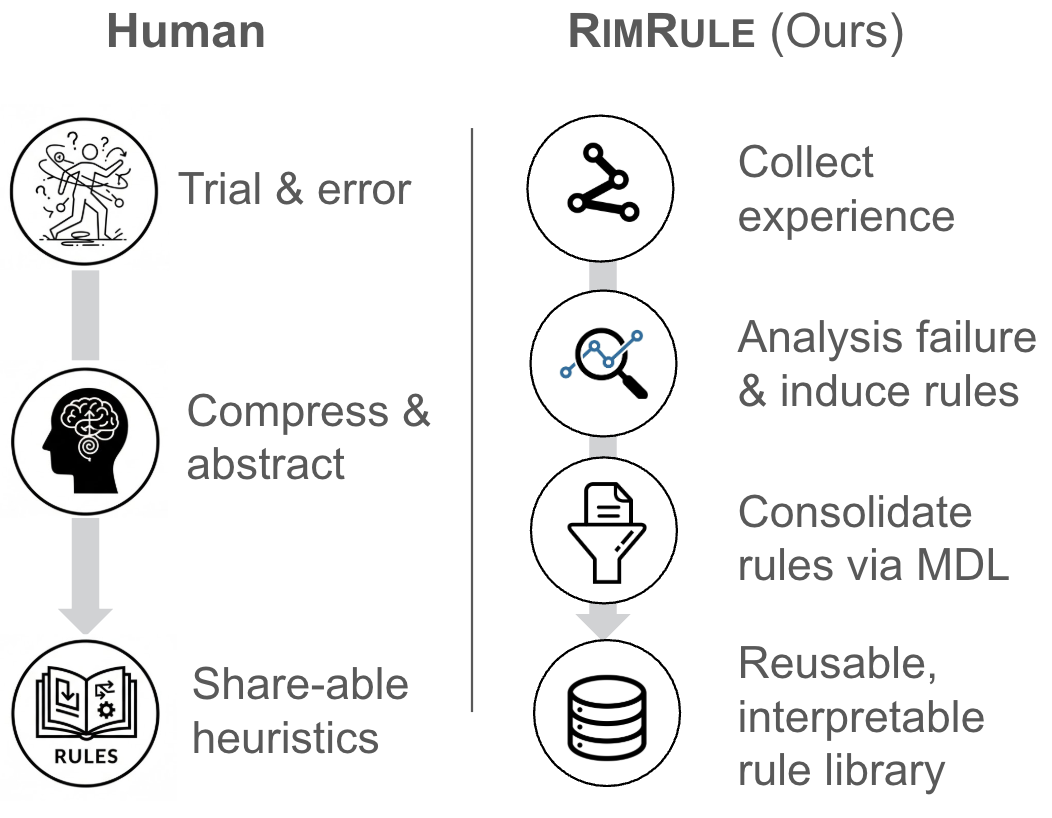
\includegraphics[width=0.85\linewidth]{figures/intro.png}
\caption{Learning reusable and interpretable rules from experience}
\label{fig:intro}
\end{figure}


Large language models (LLMs) \citep{brown2020language, bai2023qwen, team2023gemini, grattafiori2024llama} also require adaptation, especially when deployed in unfamiliar domains with specialized tools or under-documented APIs. 
However, the way LLMs adapt differs markedly from how humans do. Today, adaptation typically takes one of three forms: (i) retrieved examples for few-shot prompting~\citep{brown2020language,yizhe2021fewshot}, (ii) globally tuned prompts~\citep{pryzant2023automatic,cui2025see}, or (iii) fine-tuned model weights~\citep{hu2021lora}.
Each approach is powerful, but none supports abstraction, reuse, and interpretability in the way humans generalize from experience. Few-shot prompting reuses raw supervision but does not abstract—and LLMs often extract only shallow patterns from examples \citep{wei2023differently}; global prompts are static and brittle in interactive settings \citep{verma2024brittle}; and tuning model weights is costly, requiring retraining whenever the environment changes, 
and preventing easy sharing of acquired knowledge across models \citep{yang2024model}.


We explore a fourth paradigm for adapting LLMs—one that mirrors how humans learn from failure, as illustrated in Fig.~\ref{fig:intro}. Instead of tuning weights or retrieving demonstrations, we induce interpretable rules. At training time, these rules are proposed in response to observed failures. 
These rules are consolidated using the Minimum Description Length (MDL) principle~\citep{rissanen1978modeling,Grunwald07MDL} and stored in a dual natural-language and symbolic representation, enabling both principled compression and reliable retrieval.
At inference time, relevant rules are dynamically retrieved and injected into the prompt to improve LLM performance. 
This constitutes a distinct adaptation paradigm: unlike few-shot prompting, it emphasizes abstraction and compression over raw example replay; unlike finetuning, it produces interpretable artifacts. Because these rules are both understandable to humans and legible to modern LLMs, they can be reused across different LLMs without retraining.

%A central challenge in this paradigm is deciding which rules to keep and how to apply them. Humans do not retain every exception they encounter; instead, they consolidate experience by pruning, merging, and abstracting rules to maintain a compact, reusable knowledge base. We formalize this intuition using the Minimum Description Length (MDL) principle \citep{rissanen1978mdl,grunwald2007mdl}, which favors rule libraries that balance explanatory power with conciseness by compressing both the rules themselves and the remaining failures they explain. Effective use of such rules also requires accurate retrieval at inference time: relevant rules must be identified reliably based on the current query and available tools, while ignoring incidental linguistic variation in how rules are phrased. We therefore represent rules in a dual form—a natural-language version for interpretability and a symbolic representation that abstracts away surface-level wording, enabling principled consolidation and efficient, structure-aware retrieval.
%Ablation studies show that both components of our design are essential: MDL-guided consolidation yields more compact and effective rule libraries than prompting-based consolidation, and symbolic, structure-aware retrieval consistently outperforms retrieval based on semantic similarity over raw natural-language rules.

We demonstrate this approach on two tool-use benchmarks—ToolHop~\citep{ye2025toolhop} and BFCL~\citep{berkeley-function-calling-leaderboard}—where LLMs must reason over tool descriptions and invoke them correctly. Simple retry mechanisms based on tool error messages, or even the use of advanced long reasoning models, often fall short in reliably correcting systematic failures.
Our results highlight several key observations. 
\begin{itemize}
    \item First, inference-time rule injection consistently improves performance, including on queries involving tools that never appear in training.%, demonstrating generalization beyond surface forms.
    \item Second, learned rules transfer across LLMs in both directions: rules distilled from weaker models improve stronger, long-reasoning LLMs, and rules learned from stronger models can also benefit smaller or less capable ones.
    \item Third, our method outperforms prompting based adaptation approaches and complements finetuning, offering a distinct and synergistic axis of generalization. 
\end{itemize}
%Together, these findings indicate that compact, reusable rules can serve as a lightweight yet powerful substrate for improving LLM reasoning in tool-augmented tasks.




%This paper makes three contributions. (1) It explores an emerging fourth paradigm for LLM adaptation: compact, inference-time regularities distilled from experience and injected as step-wise guidance—mirroring how humans abstract and reuse failure corrections. (2) It introduces a principled, scalable framework for inducing and consolidating such regularities, using the Minimum Description Length (MDL) principle to balance rule complexity and correction power, and enabling distributed rule generation and canonicalized retrieval. (3) It demonstrates that this approach improves generalization to unseen tools, transfers across LLMs of varying scale and reasoning strength, and complements both few-shot learning and instruction tuning, offering a reusable and interpretable substrate for domain robustness.
